\documentclass[10pt,conference,compsocconf]{IEEEtran}

%\usepackage{times}
%\usepackage{balance}
\usepackage{url}
\usepackage{graphicx}	% For figure environment


\begin{document}
\title{Writing Scientific Papers and Software}

\author{
  Cheng Soon Ong\\
  Department of Computer Science, ETH Zurich, Switzerland
}

\maketitle

\begin{abstract}
  A critical part of scientific discovery is the
  communication of research findings to peers or the general public.
  Mastery of the process of scientific communication improves the
  visibility and impact of research. While this guide is a necessary
  tool for learning how to write in a manner suitable for publication
  at a scientific venue, it is by no means sufficient, on its own, to
  make its reader an accomplished writer. We also describe the rules
  for submission in the computational intelligence laboratory.
  This guide should be a
  starting point for further development of writing skills.
\end{abstract}

\section{Introduction}

The goal of this paper is to introduce a new road segmentation algorithm for urban areas from satellite images.
Road detection is important for several applications from autonomous driving to tracking
of road change and urban planning.
The idea of road segmentation is not a new one and has been implemente numerous times, although with
different success. The great difficulty in urban areas is the occurence of trees and cars partially blocking the
view on roads and thus making detection much harder. Additionally parking lots and railways have a lot of
identical features to roads which leads to them being missclassified.

Our approach consists of extracting 16 features from out satellite images and using those to build a machine
learing model using SVM. Our featuers consist of the original image, a smoothed version of said image and a 
skeletonization approach using an euclidean distance map to reveal the underlaying road structure.

The image preprocessing and features extraction is implemented in python with the help of numpy and cv2.
Afterwards the features are fed to matlab which is used to produce a SVM model. We decided on this 
approach because matlab is faster and easier to run on the ETH cluster. The predicted results are then
again fed to our python program for postproessing and to produce our final results.

In section XXX we describe the idea used in our approach in more detail,
followed by the implementation in sectoin XXX and results in section XXX.
Lastly we conclude the paper with a discussion of our work in section XXX and 
give ideas for future work and improvement.

\section{The Structure of a Paper}
\label{sec:structure-paper}

\begin{description}
\item[Abstract] \ \\
  Short description of the whole paper, to help the
  reader decide whether to read it.
\item[Introduction] \ \\
  Describe your problem and state your
  contributions.
\item[Models and Methods] \ \\
  Describe your idea and how it was implemented to solve
  the problem. Survey the related work, giving credit where credit is
  due.
\item[Results] \ \\
  Show evidence to support your claims made in the
  introduction.
\item[Discussion] \ \\
  Discuss the strengths and weaknesses of your
  approach, based on the results. Point out the implications of your
  novel idea on the application concerned.
\item[Summary] \ \\
  Summarize your contributions in light of the new
  results.
\end{description}


\section{Tips for Good Writing}
\label{sec:tips-writing}

The ideas for good writing have come
from~\cite{editor10,jones08,anderson04}.

\subsection{Getting Help}
One should try to get a draft read by as many friendly people as
possible. And remember to treat your test readers with respect. If
they are unable to understand something in your paper, then it is
highly likely that your reviewers will not understand it
either. Therefore, do not be defensive about the criticisms you get,
but use it as an opportunity to improve the paper. Before your submit
your friends to the pain of reading your draft, please \emph{use a
  spell checker}.

\subsection{Abstract}
The abstract should really be written last, along with the title of
the paper. The four points that should be covered~\cite{jones08}:
\begin{enumerate}
\item State the problem.
\item Say why it is an interesting problem.
\item Say what your solution achieves.
\item Say what follows from your solution.
\end{enumerate}

\subsection{Figures and Tables}

\begin{figure}[tbp]
  \centering
  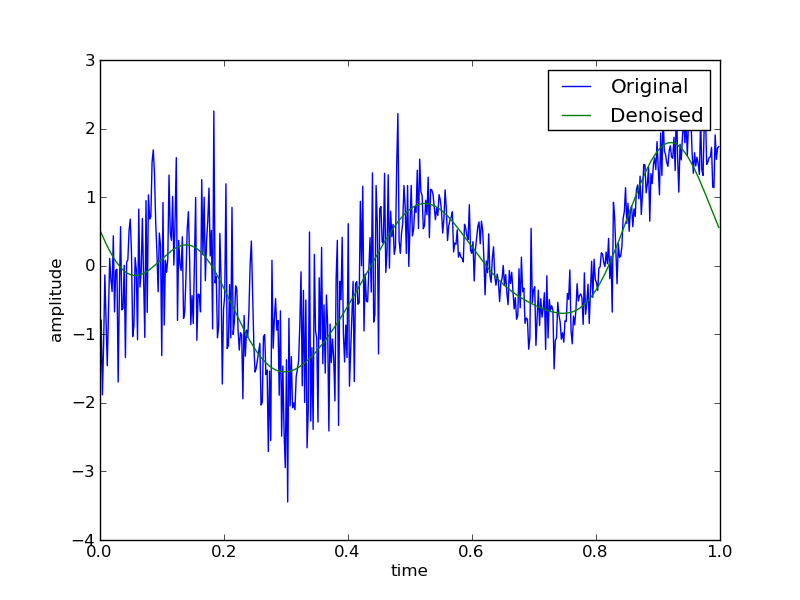
\includegraphics[width=\columnwidth]{denoised_signal_1d}
  \caption{Signal compression and denoising using the Fourier basis.}
  \label{fig:denoise-fourier}
\end{figure}
\begin{figure}[htbp]
  \centering
  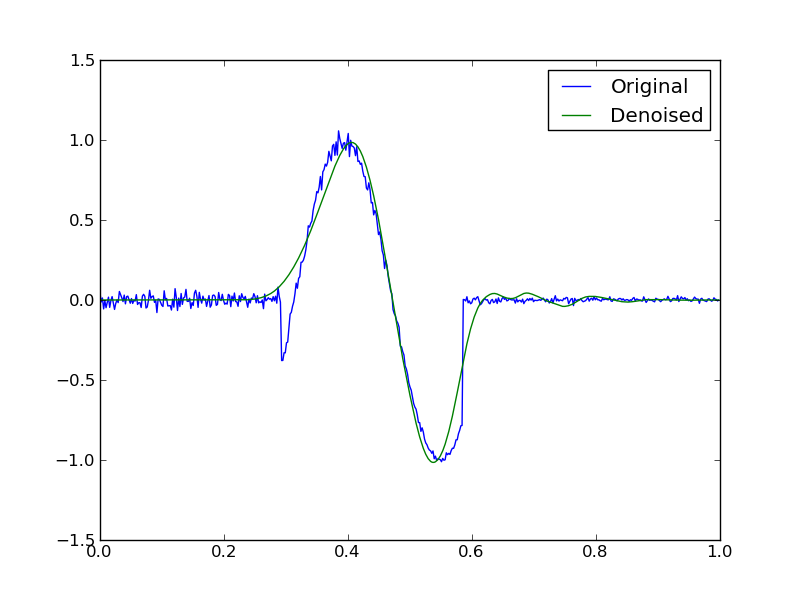
\includegraphics[width=\columnwidth]{local_wdenoised_1d}
  \caption{Signal compression and denoising using the Daubechies wavelet basis.}
  \label{fig:denoise-wavelet}
\end{figure}

Use examples and illustrations to clarify ideas and results. For
example, by comparing Figure~\ref{fig:denoise-fourier} and
Figure~\ref{fig:denoise-wavelet}, we can see the two different
situations where Fourier and wavelet basis perform well. 

\subsection{Models and Methods}
To detect roads from satellite images we decided to use support vectore machine (SVM) machine learning.
We were given 100 training images with corresponding groundtruth, which we used to classify 50 training images.

For the machine learning algorithm to be effecive we decided on a set of key features which we extracted from the training images. We do not cinsider every single pixel in the image but form patches instead. We worked with 5x5 patches, which offer a good computational speedup without loosing a lot of information of the image features.

The training and test images were taken from urban areas, which appart from roads contain mostly buildings, trees and cars. A road is a long and compared to its length thin object, often in horizontal or vertical direction and colored in a shade of grey. By concentrating on those key characteristics of a road we build a set of features which we will extract to train our model.

The first feature we use is the color. Its only natural to include this, as a road is usually grey. We can decide whether an image patch is grey by looking at its RGB values. They not only help us to find roads that look grey, but also let us recognize different object in other colors. On one of the images for example there is a pool next to a house, which naturally is blue. Naturally a blue object cannot be a road. If the values of red, blue and green all are approximately the same then the resulting color is a grey. So adding the color is a first useful feature to build our model. 

As a second feature we decided to add the standard deviation of the color. We stated earlier, that a pixel is grey, when its three RGB values are close to each others. This means that if the standard deviation is small, the red, blue and green values are all close toghether which is a strong indicator that the pixel is grey. 

After a few trial runs on the training images we noticed that there are a lot of small imperfactions which perturbe our results. Cars, trees and shadow lead to a pretty big error rate. We concluded that we have to smoothen the images to get rid of this source of noise.
We used a mean shift filter. This filter allows for edge preserving smoothing of our image. For a neighboorhod around the pixel the new spatial center and mean color value ar calculated and at the end assigned to the pixel. As parameters we used a spatial radius and a color distance of 10. Those parameters seemed to produce reasonably good results in our experiment.

We added the RGB colors and the standard deviaton of those mean shifted images as our third and fourth parameters to our feature vector. 

We wanted to have the original image but also a smoothed version with less noise. We are convinced that the combination of those two pictures are a good basis for road detection.




Out last feature is a bit more complex and is based on the paper "MORPHOLOGICAL ROAD SEGMENTATION IN URBAN AREAS FROM HIGH RESOLUTION SATELLITE IMAGES" by Gaetano, Zerubia, Scarpa and Poggi.

It is based on a morphological analysis of the image. The analysis assumes that roadsa are object that spraed over a rather large part and that have a rather small width compared to their total length. This is why a skeletonizeing algorithm is the basis for this feature. Ideally a road can be approximated and then be represented by a branch of the skeleton. 

Lets take a look at a brief overview of the algorithm. First edge detection is conducted on the image. The resuls is used to compute an eucledian distance map (EDM) which then is use to exract the skeleton from the original image. Skeletonizing is not a robust algorithm and therefore we have to improve the skeleton. Firstly the lines are thinned to 1 pixel in width. We still have to much noise though. Thus we remove small branches that are very unlikely to be part of a road. Those steps are called skeleton pruning. Finally we use double thresholding to classify skeleton branches as roads or not. We consider the average distance in the distnace map of every pixel in a skeleton branch and also the overall average distance of every pixel. In the end a watershed transform is applied to reconstruct a image full of patches, which are labeled road or not, depending from which skeleton branch they originated.




The models and methods
section should describe what was
done to answer the research question, describe how it was done,
justify the experimental design, and
explain how the results were analyzed.

The model refers to the underlying mathematical model or structure which 
you use to describe your problem, or that your solution is based on. 
The methods on the other hand, are the algorithms used to solve the problem. 
In some cases, the suggested method directly solves the problem, without having it 
stated in terms of an underlying model. Generally though it is a better practice to have 
the model figured out and stated clearly, rather than presenting a method without specifying 
the model. In this case, the method can be more easily evaluated in the task of fitting 
the given data to the underlying model.

The methods part of this section, is not a step-by-step, directive,
protocol as you might see in your lab manual, but detailed enough such
that an interested reader can reproduce your
work~\cite{anderson04,wavelab}.

The methods section of a research paper provides the information by
which a study's validity is judged.
Therefore, it requires a clear and precise description of how an
experiment was done, and the rationale
for why specific experimental procedures were chosen.
It is usually helpful to
structure the methods section by~\cite{kallet04methods}:
\begin{enumerate}
\item Layout the model you used to describe the problem or the solution.
\item Describing the algorithms used in the study, briefly including
  details such as hyperparameter values (e.g. thresholds), and
  preprocessing steps (e.g. normalizing the data to have mean value of
  zero).
\item Explaining how the materials were prepared, for example the
  images used and their resolution.
\item Describing the research protocol, for example which examples
  were used for estimating the parameters (training) and which were
  used for computing performance.
\item Explaining how measurements were made and what
  calculations were performed. Do not reproduce the full source code in
  the paper, but explain the key steps.
\end{enumerate}

\subsection{Results}

Organize the results section based on the sequence of table and
figures you include. Prepare the tables and figures as soon as all
the data are analyzed and arrange them in the sequence that best
presents your findings in a logical way. A good strategy is to note,
on a draft of each table or figure, the one or two key results you
want to address in the text portion of the results.
The information from the figures is
summarized in Table~\ref{tab:fourier-wavelet}.

\begin{table*}[htbp]
  \centering
  \begin{tabular}[c]{|l||l|l|l|}
    \hline
    Basis&Support&Suitable signals&Unsuitable signals\\
    \hline
    Fourier&global&sine like&localized\\
    wavelet&local&localized&sine like\\
    \hline
  \end{tabular}
  \caption{Characteristics of Fourier and wavelet basis.}
  \label{tab:fourier-wavelet}
\end{table*}

When reporting computational or measurement results, always
report the mean (average value) along with a measure of variability
(standard deviation(s) or standard error of the mean).


\section{Tips for Good Software}
\label{sec:tips-software}

There is a lot of literature (for example~\cite{hunt99pragmatic} and
\cite{spolsky04software}) on how to write software. It is not the
intention of this section to replace software engineering
courses. However, in the interests of reproducible
research~\cite{schwab00}, there are a few guidelines to make your
reader happy:
\begin{itemize}
\item Have a \texttt{README} file that (at least) describes what your
  software does, and which commands to run to obtain results. Also
  mention anything special that needs to be set up, such as
  toolboxes\footnote{For those who are
  particularly interested, other common structures can be found at
  \url{http://en.wikipedia.org/wiki/README} and
  \url{http://www.gnu.org/software/womb/gnits/}.}.
\item A list of authors and contributors can be included in a file
  called \texttt{AUTHORS}, acknowledging any help that you may have
  obtained. For small projects, this information is often also
  included in the \texttt{README}.
\item Use meaningful filenames, and not \texttt{temp1.m},
  \texttt{temp2.m}. The code should also unzip into a subdirectory.
\item Document your code. Each file should at least have a short
  description about its reason for existence. Non obvious steps in the
  code should be commented.
\item Describe how the results presented in your paper can potentially
  be reproduced.
\end{itemize}


\section{Computational Intelligence Laboratory Requirements}
\label{sec:cil}

Your semester project is a group effort. It consists of four parts:
\begin{enumerate}
\item The programming assignments you solve during the semester.
\item Developing a novel solution for one of the assignments, e.g. by
  combining methods from previous programming assignments into a novel
  solution.
\item Comparing your novel solution to previous assignments.
\item Writing up your findings in a short scientific paper.
\end{enumerate}

\subsection{Developing a Novel Solution}

As your final programming assignment, you develop a novel solution to
one of the four application problems. You are free to exploit any idea
you have, provided it is not identical to any other group submission
or existing Matlab implementation of an algorithm on the
internet\footnote{\url{http://www.ethz.ch/students/semester/plagiarism_s_en.pdf}}.

Two examples for developing a novel solution:
\begin{itemize}
\item You implemented a collaborative filtering algorithm based on
  dimension reduction as part of an assignment. Now you apply
  dimension reduction to inpainting.
\item You implemented both a clustering and a sparse coding algorithm
  for image compression. Now you combine both techniques into a novel
  compression method.
\end{itemize}

\subsection{Comparison to Baselines}

You compare your novel algorithm to \emph{at least two baseline
  algorithms}. For the baselines, you can use the implementations you
developed as part of the programming assignments.


\subsection{Write Up}

The submission must be in PDF form, using the \LaTeX{} template
corresponding to the IEEE style of publication. Refer to
Section~\ref{sec:latex-primer} for more information about preparing
your document. The document should be a maximum of {\bf 4 pages}.

\subsection{\LaTeX{} Primer}
\label{sec:latex-primer}

\LaTeX{} is one of the most commonly used document preparation systems
for scientific journals and conferences. It is based on the idea
that authors should be able to focus on the content of what they are
writing without being distracted by its visual presentation.
The source of this file can be used as a starting point for how to use
the different commands in \LaTeX{}. We are using an IEEE style for
this course.

\subsubsection{Installation}

There are various different packages available for processing \LaTeX{}
documents.
On Windows, use the Mik\TeX{} package (\url{http://miktex.org/}), and
on OSX use MacTeX
(\url{http://www.tug.org/mactex/2009/}). Alternatively, on OSX, you
can install the \texttt{tetex} package via
Fink\footnote{\url{http://www.finkproject.org/}} or 
Macports\footnote{\url{http://www.macports.org/}}.

\subsubsection{Compiling \LaTeX{}}
Your directory should contain at least 4 files, in addition to image
files. Images should be in \texttt{.png}, \texttt{.jpg} or
\texttt{.pdf} format.
\begin{itemize}
\item IEEEtran.cls
\item IEEEtran.bst
\item groupXX-submission.tex
\item groupXX-literature.bib
\end{itemize}
Note that you should replace groupXX with your chosen group name.
Then, from the command line, type:
\begin{verbatim}
$ pdflatex groupXX-submission
$ bibtex groupXX-literature
$ pdflatex groupXX-submission
$ pdflatex groupXX-submission
\end{verbatim}
This should give you a PDF document \texttt{groupXX-submission.pdf}.

\subsubsection{Equations}

There are three types of equations available: inline equations, for
example $y=mx + c$, which appear in the text, unnumbered equations
$$y=mx + c,$$
which are presented on a line on its own, and numbered equations
\begin{equation}
  \label{eq:linear}
  y = mx + c
\end{equation}
which you can refer to at a later point (Equation~(\ref{eq:linear})).

\subsubsection{Tables and Figures}

Tables and figures are ``floating'' objects, which means that the text
can flow around it.
Note
that \texttt{figure*} and \texttt{table*} cause the corresponding
figure or table to span both columns.


\subsection{Grading}

There are two different types of grading criteria applied to your
project, with the corresponding weights shown in brackets.
\begin{description}
\item[Competitive] \ \\
  The following criteria is scored based on your rank
  in comparison with the rest of the class.
  \begin{itemize}
  \item time taken for computation (10\%)
  \item average rank for all other criteria relevant to the task, for
    example reconstruction error and sparsity (20\%)
  \end{itemize}
  The ranks will then be converted on a linear scale into a grade
  between 4 and 6.
\item[Non-competitive] \ \\
  The following criteria is scored based on an
  evaluation by the teaching assistants.
  \begin{itemize}
  \item quality of paper (30\%)
  \item quality of implementation (20\%)
  \item creativity of solution (20\%)
  \end{itemize}
\end{description}

\subsection{Submission System}

The deadline for submitting your project report is Friday, 22 June
2012.
You need to submit:
\begin{itemize}
\item PDF of paper.
\item Archive (\texttt{.tar.gz} or \texttt{.zip}) of software. Please
  do not forget to include author information in the source archive.
\end{itemize}

\textbf{Important:} Please check the submission instructions on the webpage 
as it is the most updated instructions. 

\section{Summary}

The aim of a scientific paper is to convey the idea or discovery of
the researcher to the minds of the readers. The associated software
package provides the relevant details, which are often only briefly
explained in the paper, such that the research can be reproduced.
To write good papers, identify your key idea, make your contributions
explicit, and use examples and illustrations to describe the problems
and solutions.

\section*{Acknowledgements}
The author thanks Christian Sigg for his careful reading and helpful
suggestions.

\bibliographystyle{IEEEtran}
\bibliography{howto-paper}
\end{document}
